%% Appendix body, shared by supp.tex (separate supplement PDF) and main.tex (merged view).
%% P20 (2026-11-13): cut from 24 to <= 6 pages; the long version is archived uncompiled in
%% archive/supp_body_long_2026-11-12.tex. Every result number below is a generated macro
%% (vals.tex, supp_vals.tex, supp_perclass_vals.tex, image_vals.tex) or a generated table.

%% ============================================================================ A
\section{Setup and protocol}
\label{app:setup}

\paragraph{Streams.} We use the dataset-provided OCR and boxes of FUNSD, CORD and SROIE, page images at $224{\times}224$ and $512$ text tokens, so a LayoutLMv3 document is a sequence of $709$ positions. On CIL-CORD (\cref{tab:sessions}) a session's training and test pools keep every receipt that contains at least one of its entities, every entity of another session is labelled ``O'', and the head grows by twelve BIO tags per session; joint training uses the full-label pool, each receipt once with all its labels. Mixed alternates between new classes within a dataset and a new dataset, and its last session returns to FUNSD with all its labels and adds no tag. DIL keeps one schema \{HEADER, KEY, VALUE, OTHER\} fixed over FUNSD$\rightarrow$SROIE$\rightarrow$CORD. Every head is one linear layer; when it grows, old rows are kept and new rows are drawn from $\mathcal{N}(0,0.02^2)$.

\begin{table}[t]
\centering\scriptsize
\setlength{\tabcolsep}{2.5pt}
\caption{\textbf{Sessions.} Top: CIL-CORD (classes with the prefix of their group); pool: CORD training receipts that contain one of the session's entities ($10\%$ of each pool is held out for early stopping under the clean protocol). Bottom: Mixed; schema: the annotation scheme SBR's supervision rule reads (\cref{app:method}).}
\label{tab:sessions}
\resizebox{\linewidth}{!}{\begin{tabular}{@{}cllc@{}}
\toprule
\multicolumn{4}{@{}l}{\emph{CIL-CORD} (30 classes, 61 BIO tags)} \\
S. & Classes & & Pool \\
\midrule
1 & menu: cnt, discountprice, itemsubtotal, nm, num, price & & 800 \\
2 & menu: unitprice, vatyn, sub.cnt, sub.nm, sub.price, sub.unitprice & & 382 \\
3 & sub\_total: discount\_price, etc, othersvc\_price, service\_price, subtotal\_price, tax\_price & & 549 \\
4 & total: cashprice, changeprice, creditcardprice, emoneyprice, menuqty\_cnt, menutype\_cnt & & 723 \\
5 & total.total\_etc, total.total\_price, void\_menu.nm, void\_menu.price, sub.nm, sub.cnt & & 780 \\
\midrule
\multicolumn{4}{@{}l}{\emph{Mixed} (25 tags)} \\
S. & Dataset: tags introduced & Schema & Pool \\
\midrule
1 & FUNSD: HEADER, QUESTION & funsd & 149 \\
2 & FUNSD: ANSWER & funsd & 147--148 \\
3 & SROIE: COMPANY, DATE, ADDRESS, TOTAL & sroie & 625--626 \\
4 & CORD (super-classes): menu, sub\_total & cord & 799--800 \\
5 & CORD (super-classes): total, void\_menu, sub & cord & 797--798 \\
6 & FUNSD: none (all FUNSD labels) & funsd & 149 \\
\bottomrule
\end{tabular}}
\end{table}

\paragraph{Scoring.} A session's test labels show only its own classes, so raw scoring charges a model for every correct entity of another session and penalises it for knowing more classes. Hence, session-restricted scoring maps every predicted tag outside session $j$'s label set to ``O'' before \texttt{seqeval} span matching (for SBR after the block decision of \cref{eq:infer}); a predicted entity can then be a false positive only in its owning session and a gold entity a miss only in its own, so each error is charged at most once. However, its gap is coverage: a session's split keeps only receipts that contain one of its entities, so false positives on other receipts go uncounted. In contrast, full-label F1 scores the final model on the unmasked CORD test set and has no such gap. On every seed the order no memory (naive training, blocked readout) $<$ CoLaR $<$ memory relabelled at the boundaries $<$ \{CoLaR-SBR, SBR-Recall, memory relabelled before each session, joint training\} holds under both metrics; the MiB-style loss and ICE-O lie between CoLaR and the top group under both, and only the MiB-style loss and the boundary-relabelled memory swap places between the metrics. For CoLaR-SBR, SBR-Recall and joint training the two metrics differ by at most $\nAgreeHighMax$ points on every seed; for weak models AA is the more lenient, by $\nAgreeLowMin$ to $\nAgreeLowMax$ points without a memory and $\nAgreeColarMin$ to $\nAgreeColarMax$ for CoLaR. AA weights the five sessions equally, whereas session~1 holds $\mSessOneShare\%$ of the $\mTestSpans$ gold spans. It is noted that for the shared softmax we have span counts but no per-token outputs. Given the exact true positives and misses, full-label F1 fixes the number of false-positive spans, and (misses $-$ false positives)/misses would bound the share of missed spans labelled entirely ``O'' if every wrong span overlapped at most one missed gold span. Long runs of wrong tags break that proviso (the quantity reads up to $\mNoBankBoundMax\%$ for the blocked readout without memory, whose per-token outputs put no old entity token at ``O''), so we call it an indicator. The same count does bound CoLaR's old-span precision from below, at $\mColarOldPLb\%$ on every seed.

\paragraph{Protocol.} Under the clean protocol, we train every session in fp32 at batch size $2$ with gradient checkpointing, AdamW (learning rate $5{\times}10^{-5}$, weight decay $0.01$, clipping $1.0$), at most $10$ epochs ($100$ for joint training), and early-stop (patience $2$, $0.1$ F1 points, best weights restored) on $10\%$ held out from the session's training pool, scored with the same session restriction; the test split never selects a model. Legacy ($\dagger$) cells early-stop on the test split, differ in epoch cap by method and partly ran in fp16 mixed precision (\cref{app:baselines}). A cell switches to the clean protocol only when its three clean seeds (42, 7, 123) exist, so no cell mixes the protocols. The clean, gate and rescore runs ran one at a time on one $6$\,GB RTX 2060; some rows of the first DIL grid ran on a rented GPU.

%% ============================================================================ B
\section{Method details}
\label{app:method}

\paragraph{CoLaR.} After the first session, we freeze the embeddings and layers $1..k$, so a stored activation is produced by the same layers forever and cannot go stale. At the end of each session the layer-$k$ output of $50$ training documents is kept as the fp16 factors $(U_r\Sigma_r)$ and $V_r^{\top}$ of its truncated SVD, with the document's boxes, attention mask, labels and storing session; no raw pixels and no token ids are kept. At every step four stored documents are rebuilt, injected at layer $k{+}1$ by a forward pre-hook (their boxes and mask drive the layout biases and attention mask), and their cross-entropy is added with weight $1$; gradient checkpointing is off for the replayed pass. We count a document as $2r(709{+}768)$ bytes of factors plus $24{,}576$ bytes of boxes, mask and labels (and one byte for the session under SBR), which for the $250$ documents of CIL-CORD gives the $\nAblSbrMB$\,MB of \cref{tab:ablation} ($1$\,MB $=10^6$ bytes). The rank $r$ is the one knob that sets this size: at rank $64$ or $32$ a document would take $\nMemColarSixtyFourKB$ or $\nMemColarThirtyTwoKB$\,KB ($\nMemColarSixtyFourMB$ or $\nMemColarThirtyTwoMB$\,MB in all), computed from the same count; we make no accuracy claim for these ranks. The record the implementation holds in memory is about $1\%$ larger ($406{,}800$ against $402{,}689$ bytes per document), because it also holds the labels in the final label space; no method reads that field, only the relabelled-memory diagnostics of rung H1.

\paragraph{SBR.} A session that introduces at least one tag not yet covered opens a block with those tags, a background logit (a linear map from the $768$-dimensional head input to one logit) and its session's schema; a session that only re-annotates known tags opens none, so on DIL SBR has one block. For a document of session $s$ the supervision rule gives each block $b$ one of three modes: \emph{full} when $s$ annotates every tag of $b$ (target $y$ on $b$'s tags, $\mathrm{O}_b$ elsewhere); \emph{all-background} when $b$ belongs to another schema (target $\mathrm{O}_b$ on every token, a training-time convention that, between related receipt schemas, can call a real entity background); and \emph{skipped} otherwise. As a result, on CIL-CORD a document trains only its own block; on Mixed the all-background mode keeps a block from claiming another dataset's tokens. A stored document follows the rule of the session that stored it. At inference, with $e_b=1-p_b(\mathrm{O}_b\mid x)$ and $\tau{=}0.5$ (ties to the lower block index),
\begin{equation}
\begin{gathered}
\hat y(x)=\begin{cases}\arg\max_{t\in\mathcal{T}_{b^\star}}p_{b^\star}(t\mid x) & e_{b^\star}>\tau,\\ \mathrm{O} & \text{otherwise,}\end{cases}\\
b^\star=\arg\max_b e_b.
\end{gathered}
\label{eq:infer}
\end{equation}

\paragraph{SBR-Recall.} Every linear layer named query, key, value or dense (the attention output and both feed-forward layers) in layers $k{+}1..12$ carries one low-rank pair per delta, rank $64$ with $\alpha{=}128$, $A$ Kaiming-uniform and $B{=}0$, so a fresh delta is the identity. A rank-$64$ delta over the eight layers above $k{=}4$ has $8\times[3\cdot64\cdot1536+64\cdot1536+2\cdot64\cdot(768{+}3072)]=7{,}077{,}888$ parameters; the four deltas of CIL-CORD, counted at two bytes per parameter, give the $\nAblRecallMB$\,MB of \cref{tab:ablation} ($\nMemRecallSessMB$\,MB per session), and $\nMemRecallFpMB$\,MB ($\nMemRecallFpSessMB$\,MB per session) in fp32. The two-byte count is a reporting choice: the deltas were trained and evaluated in fp32, and no run evaluated half-precision deltas. The first session trains the base; after that, the encoder is frozen and only the head, the background weights and the current delta train. The loss groups a document's blocks by the delta each is read under and runs one forward pass per distinct delta, so every term is computed under its block's own trunk state, as is inference (five passes on CIL-CORD; a cached implementation repeats only the $12-k$ upper layers, about $3.7$ layer-equivalents of one pass). Without a memory on one schema a later session's loss contains only its own block, so an old block's delta and background weights are outside the graph and its rows of the tag head get zero gradient; only AdamW's decoupled weight decay (under $1\%$ over a run) and out-claiming by new blocks can move its tokens. In the clean runs no session falls more than $\nRecallMaxLoss$ points below its diagonal at any later boundary.

\begin{table*}[t]
\centering\scriptsize
\setlength{\tabcolsep}{4pt}
\caption{\textbf{Memory accounting} (CIL-CORD: $250$ stored documents, or four deltas; $1$\,MB $=10^6$ bytes). Computed: the size of an encoding no run used, from the counts in the text. Trainable: parameters trained at once after session~1 (SBR-Recall: one delta at a time, four over the run); peak GPU memory and hours per run from the clean runs ($^{n=k}$: only $k$ uninterrupted runs timed). Generated.}
\label{tab:memory}
% AUTO-GENERATED by scripts/rca/make_clean_tables.py -- do not edit.
\begin{tabular}{@{}lcccccccc@{}}
\toprule
Storage form & Per unit & Total MB & Pixels & Token ids & Full-label F1 & Trainable (M) & Peak GPU MB & h/run \\
\midrule
Layer-4 latent, fp16, uncompressed (computed) & 1113.6\,KB/doc & 278.4 & no & no & -- & -- & -- & -- \\
Raw document as held (fp32 pixels) & 630.8\,KB/doc & 157.7 & yes & yes & $88.4{\pm}1.0$ & 125.4 & 2666 & 2.9 \\
Raw document, 8-bit pixels (computed) & 179.2\,KB/doc & 44.8 & yes & yes & -- & -- & -- & -- \\
CoLaR rank 128 & 402.7\,KB/doc & 100.7 & no & no & $89.1{\pm}2.0$ & 56.8 & 2436 & 2.0$^{n=1}$ \\
CoLaR rank 32 & 119.1\,KB/doc & 29.8 & no & no & $27.4{\pm}2.5$ & 56.8 & 2436 & 2.2 \\
SBR-Recall deltas, fp16 (computed) & 14.2\,MB/session & 56.6 & no & no & -- & -- & -- & -- \\
SBR-Recall deltas, fp32, as trained & 28.3\,MB/session & 113.2 & no & no & $92.6{\pm}1.0$ & 7.1 & 2436 & 1.7 \\
\bottomrule
\end{tabular}

\end{table*}

\paragraph{Memory accounting (\cref{tab:memory}).} We count a raw-replay document as our code holds it: $3\cdot224^2$ pixels at four bytes (one byte in the 8-bit row, which no run used) and $512\cdot7{+}1$ int64 values (per token its id, four box coordinates, mask and label; one for the session). The uncompressed latent is $709\cdot768$ fp16 values plus the $24{,}576$ bytes of the CoLaR record. Raw replay with the blocked readout trains the whole network (a raw memory could freeze the same layers; ours does not); CoLaR and SBR-Recall train only what lies above layer~$4$ after session~1, and CoLaR replays a document through the upper eight layers only. Wall-clock is reported for completeness: only one CoLaR-SBR run ran uninterrupted, so we do not compare run times.

%% ============================================================================ C
\section{Baselines}
\label{app:baselines}

\begin{table*}[t]
\centering\scriptsize
\setlength{\tabcolsep}{3pt}
\caption{\textbf{Baseline card} (the methods of \bodyref{tab:main}{the main paper's comparison table}). What our port changes against the published method, what it keeps across sessions, and the number of seeds behind each cell ($\dagger$: legacy protocol). Legacy cells early-stop on the session's test split; their epoch cap is $100$ for ER, DER++, LwF, CPFD and IS3, $30$ for CODA-Prompt and CL-LoRA and $10$ for LCA and the CoLaR family; most ran in fp16 mixed precision, but IS3 and LCA always in fp32, and seed 42 of several CIL-CORD baselines in fp32, so some cells mix precisions across seeds. LwF excludes one fp16 seed per scenario that collapsed to all-background. The first DIL grid saved no configuration; its settings are the grid script's defaults. Generated.}
\label{tab:baselinecard}
% AUTO-GENERATED by scripts/rca/make_clean_tables.py -- do not edit.
\begin{tabular}{@{}l>{\raggedright\arraybackslash}p{1.9cm}>{\raggedright\arraybackslash}p{7.4cm}>{\raggedright\arraybackslash}p{3.1cm}ccc@{}}
\toprule
 & & & & \multicolumn{3}{c}{Seeds} \\
\cmidrule(l){5-7}
Method & Family & What our port changes & Memory & CIL-CORD & Mixed & DIL \\
\midrule
ER & Replay & -- & 200 raw documents & 3$^{\dagger}$ & 2$^{\dagger}$ & 3$^{\dagger}$ \\
DER++ & Replay & -- & 200 raw documents + logits & 3$^{\dagger}$ & 2$^{\dagger}$ & 3$^{\dagger}$ \\
LwF & Regularisation & -- & previous model & 2$^{\dagger}$ & 1$^{\dagger}$ & 3$^{\dagger}$ \\
CODA-Prompt & Prompt, LoRA & prompts prepended to the input sequence (an input-prepend variant) & none (prompt pool) & 2$^{\dagger}$ & 2$^{\dagger}$ & 3$^{\dagger}$ \\
CL-LoRA & Prompt, LoRA & one shared rank-8 adapter retrained each session (published: random-orthogonal shared and block-wise task-specific adapters, early-exit distillation); gradient reassignment at scale 1, i.e.\ off & previous model, past adapter matrices & 2$^{\dagger}$ & 2$^{\dagger}$ & 3$^{\dagger}$ \\
CPFD & Continual NER & one growing token head (published: per-task classifiers); sample weights set to 1 & previous model & 2$^{\dagger}$ & 2$^{\dagger}$ & 3$^{\dagger}$ \\
IS3 & Continual NER & one growing token head (published: per-task classifiers) & previous model, class prototypes & 2$^{\dagger}$ & 2$^{\dagger}$ & 1$^{\dagger}$ \\
LCA & Merging & one growing token head (published: per-task heads); Gaussians per token class, ``O'' excluded & base and per-session backbones, class Gaussians & 2$^{\dagger}$ & 2$^{\dagger}$ & 3$^{\dagger}$ \\
\bottomrule
\end{tabular}

\end{table*}

\paragraph{Ports.} We port every baseline onto the one growing token head that every other row uses (\cref{tab:baselinecard}); none is checked against its published NER numbers. Hyper-parameters are the methods' defaults as recorded by each run: ER and DER++ keep a reservoir of $200$ documents (DER++ $\alpha{=}\beta{=}0.5$), LwF uses $T{=}2$, CL-LoRA a rank-$8$ adapter with an orthogonality penalty of $0.5$. LCA keeps its published optimiser instead of our AdamW recipe: SGD with momentum $0.9$, a cosine schedule, learning rate $0.01$ and weight decay $5{\times}10^{-4}$, and SGD at $5{\times}10^{-3}$ for the realignment. Rows marked $^{p}$ in \bodyref{tab:main}{the comparison table of the main paper} were made before we fixed the order of the adapter matrices in our ports' orthogonality penalty.

\paragraph{How the set was fixed.} We fixed the set after a first grid on all three streams. There, EWC~\citep{kirkpatrick2017ewc}, L2P~\citep{wang2022l2p} and DualPrompt~\citep{wang2022dualprompt} left at least sessions~4 and~5 of CIL-CORD unlearned on every seed, and ER with SAM (our C-Flat++ port, run with its curvature weight at $0$) stayed within $\nSamErGapMax$ AA of ER on every seed, so these were dropped; O-LoRA~\citep{wang2023olora} was dropped because its runs predate the penalty fix. Methods that fail on the scenario (CPFD, IS3) were kept. Four baselines end below naive training on every seed because they learn later sessions poorly: CPFD learns no session after the first (at most $\nCpfdLateMax$ F1 on a later diagonal), and IS3, CODA-Prompt and LCA each learn some later session to at most $\nBaseWorstLateMax$ F1, where naive training learns every session to at least $\nNaiveDiagMin$.

%% ============================================================================ D
\section{Extended results and ablations}
\label{app:results}

\begin{figure*}[t]\centering
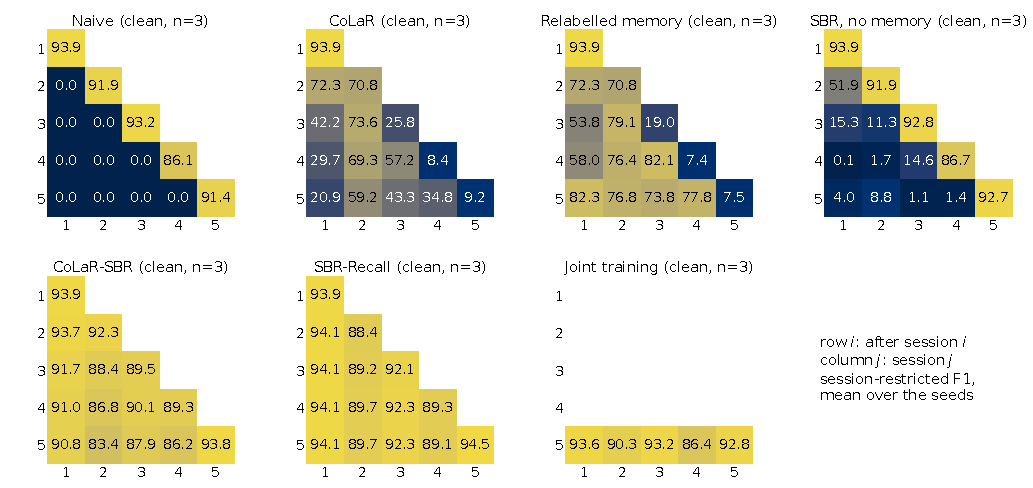
\includegraphics[width=0.92\linewidth]{figures/heatmaps.pdf}
\caption{\textbf{Retention matrices} (CIL-CORD, LayoutLMv3, clean protocol, session-restricted F1, mean over the three seeds). Row $i$: after training session $i$; column $j$: session $j$. Joint training is one pooled run, so only its final row exists.}
\label{fig:heatmaps}\end{figure*}

\paragraph{Retention (\cref{fig:heatmaps}).} We read the diagonal (each session when it is learned) and the bottom row (the final model). Naive training learns every session and keeps none of the earlier ones. CoLaR keeps part of the old sessions; however, from session~3 on its diagonal is low: the session being trained is suppressed (rung H0). With the relabelled memory sessions~3 and~4 rise one boundary after they are learned, while the last session stays low (rung H1). The blocked readout without a memory learns every session and loses the old ones; in contrast, with the memory the columns hold. \emph{Where the remaining gap lies:} under CoLaR-SBR a column loses $\sbrLossMin$ to $\sbrLossMax$ points from its diagonal to the final row of the mean matrix, session~$\sbrLossMaxSession$ the most, and under SBR-Recall every column of the mean matrix ends within $\recallDevMax$ points of its diagonal, so what CoLaR-SBR still loses to joint training is retention of early sessions, which per-session deltas remove on this stream.

\begin{figure*}[t]\centering
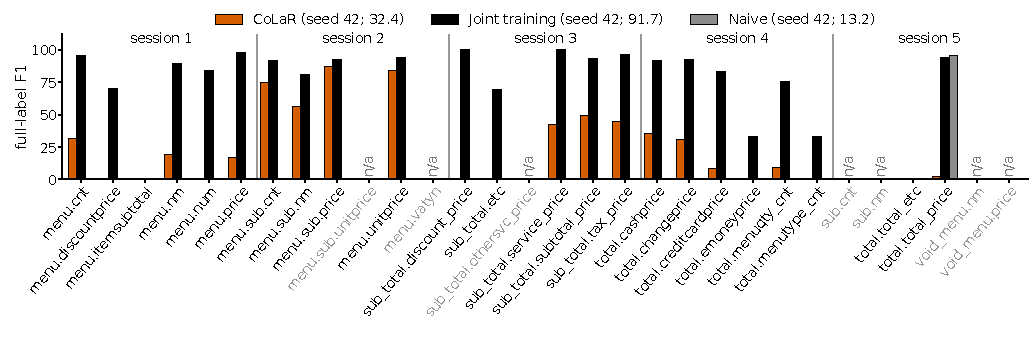
\includegraphics[width=0.92\linewidth]{figures/perclass.pdf}
\caption{\textbf{Per-class full-label F1} of four prediction-dump re-runs (CIL-CORD, final model, unmasked test set; seed 42 only, each reproducing the full-label F1 of its clean run, given in the legend). Classes grouped by the session that introduces them; grey: the class does not occur in the test set.}
\label{fig:perclass}\end{figure*}

\paragraph{Per class (\cref{fig:perclass}).} It is noted that the dump re-runs are not table cells, and every statement here is about seed 42 only. Of the $\pcPresent$ classes that occur in the test set, the joint-training re-run finds $\pcFoundJoint$ (F1 above $0$), the CoLaR-SBR re-run $\pcFoundSbr$, the CoLaR re-run $\pcFoundColar$ and the naive re-run $\pcFoundNaive$; $\pcBothMissed$ of the classes the CoLaR-SBR re-run misses are missed by joint training too. In the CoLaR re-run the session-5 classes are almost never found (the suppressed newest session) and the session-1 classes, which hold most test entities, are found only in part, while several session-2 and session-3 classes are kept.

\begin{table}[t]
\centering\scriptsize
\setlength{\tabcolsep}{2pt}
\caption{\textbf{Component ablations on CIL-CORD}, the runs of \bodyref{tab:ladder}{the ladder table of the main paper} (clean protocol, LayoutLMv3, mean $\pm$ s.d. over three seeds). Ticks: memory (Mem.; latent unless marked raw), blocked readout (Blk.), per-session deltas ($\Delta$), true labels (True). All rows but naive, joint and the raw memory freeze at least the embeddings and layers $1..4$ after session~1. MB: bytes kept across sessions (\bodyref{sec:cost}{the main paper's memory-cost section}); SBR-Recall's deltas at two bytes per parameter, a reporting choice ($\nMemRecallFpMB$ as trained in fp32). $^{r}$Stored documents given their true labels (H1): the older ones at each boundary, or all of them before each session (pre-session).}
\label{tab:ablation}
% AUTO-GENERATED by scripts/rca/make_clean_tables.py -- do not edit.
\begin{tabular}{@{}lccccccc@{}}
\toprule
Configuration & Mem. & Blk. & $\Delta$ & True & Full-label F1 & AA & MB \\
\midrule
Naive &  &  &  &  & $13.0{\pm}0.2$ & $18.3{\pm}0.5$ & 0 \\
\midrule
+ memory (CoLaR) & $\checkmark$ &  &  &  & $30.7{\pm}1.5$ & $33.5{\pm}1.0$ & 100.7 \\
+ blocked readout &  & $\checkmark$ &  &  & $11.4{\pm}2.3$ & $21.6{\pm}2.2$ & 0 \\
+ both (CoLaR-SBR) & $\checkmark$ & $\checkmark$ &  &  & $89.1{\pm}2.0$ & $88.4{\pm}2.6$ & 100.7 \\
SBR-Recall &  & $\checkmark$ & $\checkmark$ &  & $92.6{\pm}1.0$ & $91.9{\pm}0.6$ & 56.6 \\
\midrule
Relabelled memory$^{r}$ & $\checkmark$ &  &  & $\checkmark$ & $76.5{\pm}2.3$ & $63.6{\pm}1.9$ & 100.9 \\
Joint (reference) &  &  &  & $\checkmark$ & $92.0{\pm}0.4$ & $91.3{\pm}0.8$ & -- \\
\bottomrule
\end{tabular}

\end{table}

\begin{figure}[t]\centering
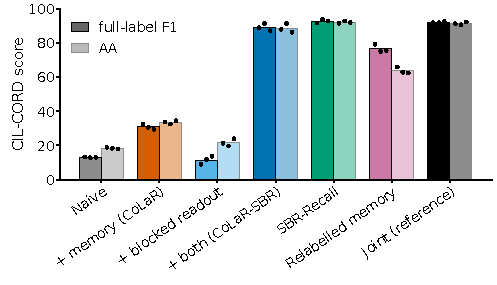
\includegraphics[width=\linewidth]{figures/ablation.pdf}
\caption{\textbf{The component grid of \cref{tab:ablation}} (CIL-CORD, clean protocol; bar: mean of three seeds, dots: the seeds; full-label F1 dark, AA light).}
\label{fig:ablation}\end{figure}

\begin{table}[t]
\centering\scriptsize
\setlength{\tabcolsep}{3pt}
\caption{\textbf{Design-choice ablations} (fp32 gate runs$^\dagger$: $10$-epoch cap, test-split early stopping, session-restricted scoring; AA per seed when fewer than three, else mean $\pm$ s.d.). The last two columns give the lowest diagonal entry (a session when learned) and the lowest final-row entry over every session and seed of the row. Generated.}
\label{tab:ablext}
% AUTO-GENERATED by scripts/rca/make_clean_tables.py -- do not edit.
\begin{tabular}{@{}lccc@{}}
\toprule
Variant & AA & min $R[j,j]$ & min $R[T,j]$ \\
\midrule
\multicolumn{4}{@{}l}{\emph{SBR-Recall delta capacity, CIL-CORD}} \\
\quad rank 8, Q/K/V, with memory & $80.5^{\dagger}$ & 61.5 & 63.2 \\
\quad rank 8, Q/K/V, no memory & $82.5^{\dagger}$ & 64.9 & 66.4 \\
\quad rank 64, Q/K/V + dense, no memory & $92.8{\pm}0.5^{\dagger}$ & 88.8 & 88.6 \\
\midrule
\multicolumn{4}{@{}l}{\emph{SBR-Recall across schemas, Mixed (rank 64)}} \\
\quad no memory & $44.7^{\dagger}$ & 82.0 & 0.0 \\
\quad $50$-document memory & $85.9^{\dagger}$ & 81.2 & 75.0 \\
\midrule
\multicolumn{4}{@{}l}{\emph{Head slots on CoLaR-SBR, CIL-CORD}} \\
\quad CoLaR-SBR & $88.0{\pm}2.0^{\dagger}$ & 85.9 & 72.8 \\
\quad + LexSlot & $89.7{\pm}0.5^{\dagger}$ & 89.8 & 80.6 \\
\bottomrule
\end{tabular}

\end{table}

\paragraph{Design choices (\cref{fig:ablation,tab:ablext}).} \Cref{fig:ablation} draws the component grid with its seeds; \cref{tab:ablext} gathers the design-choice runs, all legacy gate runs and mostly single seeds, so each is compared only within its own protocol. \emph{Delta capacity.} At rank $8$ on query, key and value, SBR-Recall learns its weakest session (the sub-total and total fields, mostly prices) only to the value in the min $R[j,j]$ column, and adding the memory does not help; at rank $64$ with the attention output and feed-forward layers every session is learned on all three seeds. Hence, isolation was sound at rank $8$, and the capacity of the delta was the limit. Rank $64$ is the one setting we chose on CIL-CORD, from these legacy runs, before the clean re-runs. \emph{Across schemas.} Without a memory on Mixed, an old block is trained towards its background on every token of another schema's documents and nothing trains it towards its own tags, so its blocks fall silent until their domain returns and at least one session ends at zero; the trunk is frozen, so this is a readout effect, not drift. In contrast, the $50$-document memory supplies the positive counterweight: no session ends below the value in the last column, and isolation by deltas does not replace the memory across schemas (one seed). \emph{Head slots.} LexSlot adds head slots that a session updates only when its OCR vocabulary selects them, and stores token ids, unlike CoLaR. Stacked on CoLaR-SBR it raises the gate mean and narrows the spread between seeds; we keep it as a row, not a method.

%% ============================================================================ E
\section{Drift evidence}
\label{app:drift}

\begin{table}[t]
\centering\scriptsize
\setlength{\tabcolsep}{3pt}
\caption{\textbf{Drift and its remedy on four encoders} (DIL, AA, mean $\pm$ s.d. over three seeds; first grid, legacy protocol$^\dagger$). On average, replay comes within one point of joint training or exceeds it, and EWC and LwF stay within ten points of naive training. ``--'': did not fit the $6$\,GB GPU. Generated.}
\label{tab:dil}
\resizebox{\linewidth}{!}{% AUTO-GENERATED by scripts/rca/make_clean_tables.py -- do not edit.
\begin{tabular}{lcccccc}
\toprule
Backbone & Naive & EWC & LwF & ER & DER++ & Joint \\
\midrule
LayoutLMv3 & $41.3{\pm}1.5$ & $41.2{\pm}1.1$ & $43.7{\pm}1.1$ & $87.9{\pm}1.4$ & $88.0{\pm}0.9$ & $88.7{\pm}1.1$ \\
LiLT & $40.1{\pm}0.5$ & $48.4{\pm}5.9$ & -- & $85.7{\pm}0.5$ & $84.4{\pm}0.3$ & $83.8{\pm}1.2$ \\
BROS & $40.3{\pm}1.8$ & $45.0{\pm}4.9$ & $35.1{\pm}3.1$ & $87.8{\pm}0.4$ & $87.5{\pm}1.1$ & $87.5{\pm}1.3$ \\
BERT & $39.4{\pm}0.3$ & $46.6{\pm}3.0$ & $40.5{\pm}0.1$ & $77.1{\pm}0.9$ & $77.4{\pm}0.6$ & $77.2{\pm}0.4$ \\
\bottomrule
\end{tabular}
}
\end{table}

\begin{figure}[t]\centering
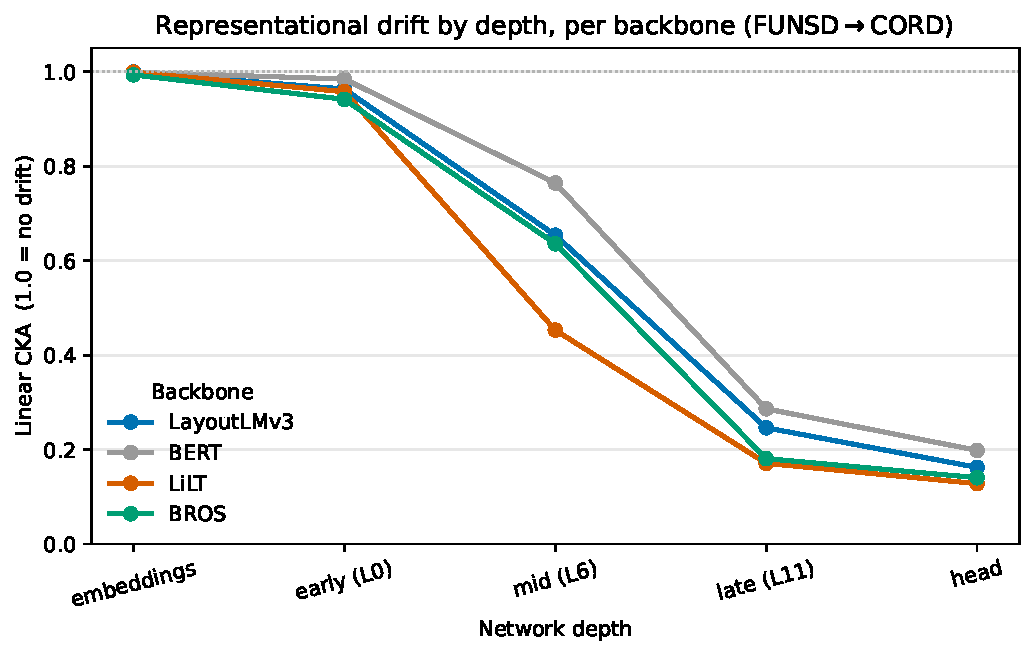
\includegraphics[width=0.9\linewidth]{figures/backbone_cka_gradient.pdf}
\caption{\textbf{Drift by depth}: linear CKA between checkpoints before and after the second task (FUNSD$\rightarrow$CORD, each dataset with its own labels) under naive fine-tuning on four encoders ($1.0$: no drift; three seeds).}
\label{fig:cka}\end{figure}

\paragraph{Where drift sits.} We observe that under naive fine-tuning on a fixed label space every encoder forgets its earlier domains (\cref{tab:dil}). On our pilot stream FUNSD$\rightarrow$CORD$\rightarrow$SROIE, where each dataset brings its own labels, the representation drift grows with depth on all four encoders, largest at the head and the last layer and smallest at the embeddings (\cref{fig:cka}). That forgetting concentrates in the output-facing computation is known for image classifiers~\citep{ramasesh2021anatomy}; here it holds, on that stream, for three multimodal document encoders and a text-only one. On images the readout can also be repaired from class statistics (\cref{app:image}); on token-labelled documents, in our experiments, only old-task supervision of the readout repaired it.

\paragraph{Replay against the classical remedies.} On every encoder of \cref{tab:dil} replay (ER, DER++) comes close to joint training on average, whereas EWC and LwF stay near naive training; the benefit of EWC over naive training differs between encoders while the cause does not, which is why the table reports four. The buffer-free alternatives we built or ported for this drift each failed for a reason identified per boundary, in mostly single-seed diagnostics at their own operating points: head merging (TIES or Fisher) is close to a no-op; merging with Gaussian classifier realignment (LCA, three seeds) halves backward transfer but stops acquisition; subspace transfer (HGT, CUBER) trades stability for plasticity at the naive level; head slots without a buffer cannot re-ground the shared head; feature-Gaussian replay recovers only the densely labelled task, because a marginal summary breaks whole-document consistency; and refreshing stored labels with the model's own predictions is a no-op, because the model is confident on almost no stale ``O'' token.

%% ============================================================================ F
\section{Image classification}
\label{app:image}


\begin{table}[t]
\centering\scriptsize
\setlength{\tabcolsep}{3pt}
\caption{\textbf{Image class-incremental learning} (AA, mean $\pm$ s.d., seeds 42/7/123). CIFAR-100 and ImageNet-R in ten sessions (class order seed $1993$, as in SLCA and RanPAC); ViT-B/16 pre-trained on ImageNet-21k with a linear head on the CLS token. House recipe, not the clean document protocol: AdamW at $5{\times}10^{-5}$ (SLCA and LCA: SGD at $0.01$), batch size $16$, epoch cap $100$ (SLCA: $20$) with early stopping, fp32 with gradient checkpointing (the latent memory and CoLaR: mixed precision). ER and DER++ keep $2{,}000$ raw images, SLCA class Gaussians, the latent memory and CoLaR $500$ images per session as layer-4 latents ($5{,}000$ after ten sessions). SLCA and RanPAC take the slots CPFD and IS3 take on documents. $^{v}$Diagnostic probe on seed-42 variant runs (on CIFAR-100 a second run of the latent memory, on ImageNet-R a CoLaR run with a $20$-epoch cap): a ridge readout refit on all training data through the run's adapted trunk; not a method. Generated.}
\label{tab:image}
\resizebox{\linewidth}{!}{% Row labels hand-patched on 2026-11-11 (terminology); numbers unchanged.
% Auto-generated by scripts/rca/make_image_table.py (do not edit by hand).
% Metric: AA (mean $\pm$ std over seeds 42/7/123); ``pending'' = not all seeds on disk yet.
\begin{tabular}{lcc}
\toprule
\textbf{Method} & \textbf{CIFAR-100} & \textbf{ImageNet-R} \\
\midrule
Naive & 11.7\;{\scriptsize $\pm$ 1.1} & 9.3\;{\scriptsize $\pm$ 0.3} \\
LwF & 15.7\;{\scriptsize $\pm$ 0.6} & 12.7\;{\scriptsize $\pm$ 1.4} \\
ER (2{,}000 exemplars) & 76.2\;{\scriptsize $\pm$ 1.2} & 54.8\;{\scriptsize $\pm$ 0.7} \\
DER++ (2{,}000 exemplars) & 76.5\;{\scriptsize $\pm$ 1.5} & 52.8\;{\scriptsize $\pm$ 1.1} \\
CODA-Prompt & 15.2\;{\scriptsize $\pm$ 1.8} & 8.4\;{\scriptsize $\pm$ 0.7} \\
CL-LoRA (2025) & 14.1\;{\scriptsize $\pm$ 1.2} & 11.4\;{\scriptsize $\pm$ 0.8} \\
SLCA (2023) & 87.5\;{\scriptsize $\pm$ 0.2} & 65.0\;{\scriptsize $\pm$ 0.3} \\
RanPAC (2023) & 85.3\;{\scriptsize $\pm$ 0.1} & 58.5\;{\scriptsize $\pm$ 0.3} \\
LCA (2026) & 77.2\;{\scriptsize $\pm$ 3.2} & 54.7\;{\scriptsize $\pm$ 3.6} \\
\midrule
\textbf{Latent memory, 500/class (ours, uncompressed)} & 80.0\;{\scriptsize $\pm$ 0.7} & 55.1\;{\scriptsize $\pm$ 1.3} \\
\textbf{CoLaR $r{=}128$, 500/class (ours)} & 79.5\;{\scriptsize $\pm$ 1.0} & 55.3\;{\scriptsize $\pm$ 1.4} \\
Ridge readout on the latent-memory trunk (probe, seed 42) & 88.3 & 72.3 \\
\midrule
Joint training (reference) & 89.5\;{\scriptsize $\pm$ 0.4} & 77.6\;{\scriptsize $\pm$ 0.5} \\
\bottomrule
\end{tabular}
}
\end{table}

\paragraph{What transfers, and what does not.} SLCA~\citep{zhang2023slca} and RanPAC~\citep{mcdonnell2023ranpac} lead on both datasets, above the latent memory and CoLaR on every seed, and we make no state-of-the-art claim on images; our recipe is not SLCA's published one, and our SLCA and joint-training numbers are below the published ones. The latent memory is competitive with raw replay at $2.5\times$ the items: on CIFAR-100 the latent memory and CoLaR are above ER and DER++ with $2{,}000$ raw images on every seed, and on ImageNet-R they are within $\imgBankErGapImnr$ and $\imgColarErGapImnr$ points of ER on every seed. They store no pixel but more items ($\imgBankMB$ and $\imgColarMB$\,MB as recorded, against $\imgErTwoKMB$\,MB for $2{,}000$ raw images as our buffer stores them), and replay with $200$ raw images falls to $\imgErTwoHCifar$ / $\imgErTwoHImnr$ (ER). Compressing each stored latent to rank $128$ moves AA by at most $\imgColarBankGapMax$ points on any seed. SLCA's margin comes from its classifier alignment: without it the same recipe falls to $\imgSlcaNocaCifar$ / $\imgSlcaNocaImnr$. On the one-seed variant runs of the probe row, the adapted trunk supports a readout above every seed of the latent memory and CoLaR rows, so the trunk holds more than the trained head reads out, the head-locus reading of documents; this rests on one seed. Since an image carries one label and has no background class, there is no background conflict to remove: SBR is not run on images, and a stored image's label never goes stale. With a plain softmax head CoLaR reaches $\imgColarCifar$ / $\imgColarImnr$ against $\imgJointCifar$ / $\imgJointImnr$ for joint training, whereas on CIL-CORD the same memory with a shared softmax reaches $\nColar$ AA against $\nJoint$, a much larger gap, consistent with a cause that only token labelling has.
